\section{Positive and Unlabeled Learning}
\label{sec:pulearning}

\textit{One sentence summary of Positive and Unlabeled Learning}

%%%%%%%% TEXT PU Learning setup

\paragraph{Formulation}

\textit{This part should explain the Positive and Unlabeled Learning setup with mathematical representation when necessary.}


%%%%%%%% TEXT Modeling
% \paragraph{Class weight}
\textit{This part should discuss the linear model for observing positive conditioning on true positive and its relationship to changing the class weight.}


%%%%%%%% TEXT Imbalanced
\textit{This part should explain the influence of the imbalanced problem and how to overcome.}


%%%%%%%% TEXT Exponential loss
\textit{This part should explain why the exponential loss could perform better than the cross-entropy loss, potentially with a figure of 2D Gaussians.}


%%%%%%%% TEXT Expontial loss FADE IN
\textit{This paragraph should explain why fade-in was introduced to avoid all-positive prediction}




%%%%%%%% FIGURE MOONS
\begin{figure*}
\begin{center}
% \fbox{\rule{0pt}{2in} \rule{.9\linewidth}{0pt}}
   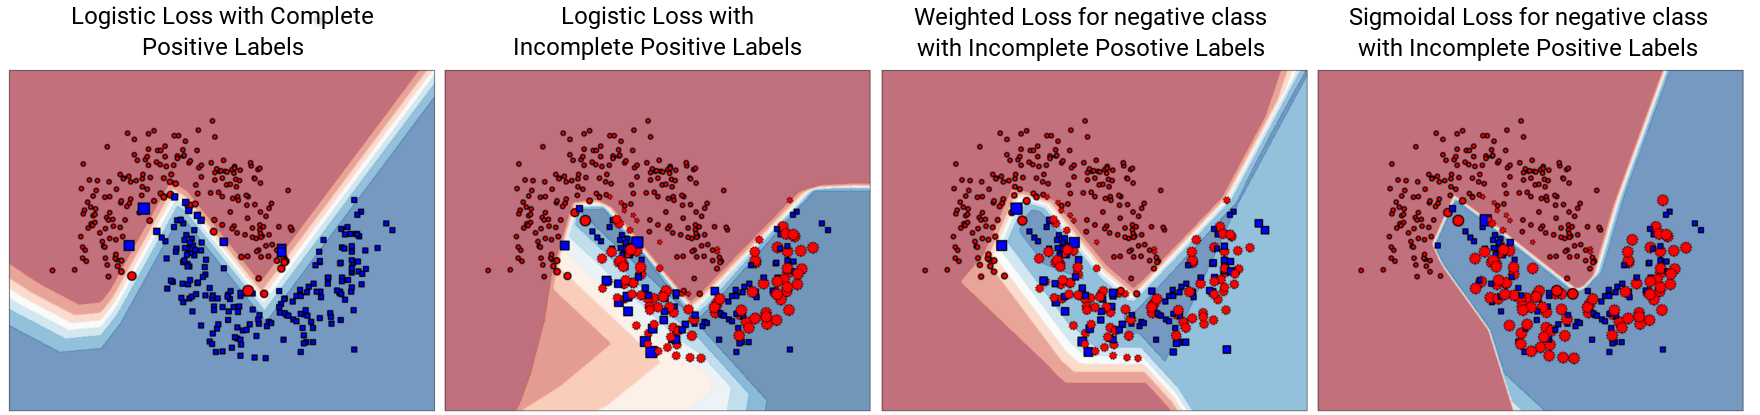
\includegraphics[width=0.95\linewidth]{img/moons.png}
\end{center}
   \caption{MOONS}
\label{fig:moons}
\end{figure*}


%%%%%%%% FIGURE Losses
\begin{figure}[t]
\begin{center}
% \fbox{\rule{0pt}{2in} \rule{0.9\linewidth}{0pt}}
   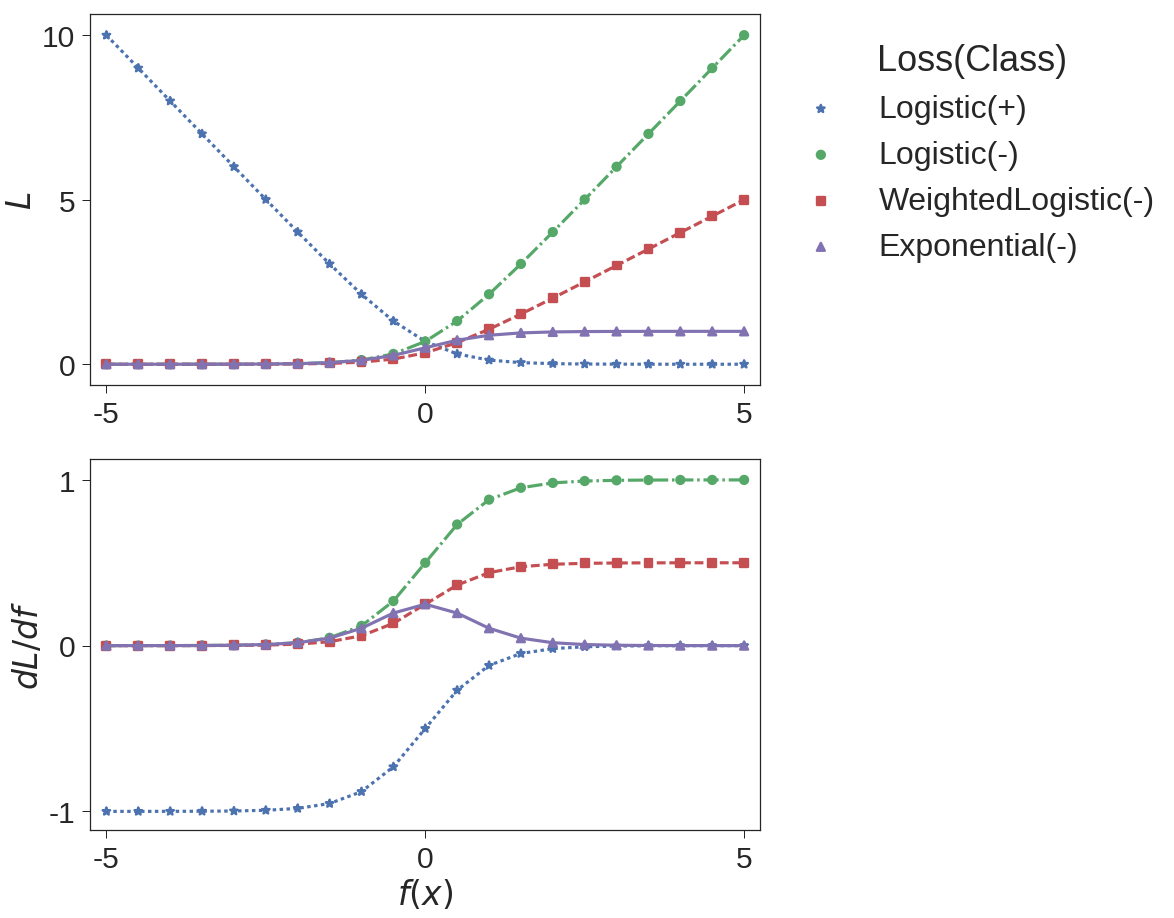
\includegraphics[width=0.95\linewidth]{img/losses.png}
\end{center}
   \caption{The Logistic Loss, Weighted Logistic Loss, Exponential Loss and their dirivatives.}
\label{fig:losses}
\end{figure}


%%%%%%%% FIGURE Varying positive annotating percetage
\begin{figure}[t]
\begin{center}
\fbox{\rule{0pt}{2in} \rule{0.9\linewidth}{0pt}}
  %  \includegraphics[width=0.95\linewidth]{img/}
\end{center}
   \caption{VGG8 CIFAR10 with 10\%, 20\%, 50\%, 80\% and 100\% of the positive examples annotated}
\label{fig:percentage}
\end{figure}

%%%%%%%% TABLE CIFAR10
\begin{table}
\begin{center}
\begin{tabular}{ll|llll}
Annotation  & Loss & acc. & prec. & rec. & $F_1$ \\
\hline
Complete    & CrossEntropyU    & 0.87 & 0.88 & 0.82 & 0.85 \\
50\%P+50\%N & CrossEntropyU    & 0.83 & 0.84 & 0.78 & 0.80 \\
50\%P+U     & CrossEntropyU    & 0.61 & 0.92 & 0.30 & 0.38 \\
50\%P+U     & WeightedU        & 0.66 & 0.93 & 0.39 & 0.51 \\
50\%P+U     & ExponentialU     & 0.82 & 0.86 & 0.73 & 0.78 \\
50\%P+U     & BootstrapHard    & 0.74 & 0.81 & 0.60 & 0.67 \\
50\%P+U     & LinearNoiseModel & & & & \\
50\%P+U     & DropoutRegularization & & & & \\
\end{tabular}
\end{center}
\caption{VGG8 CIFAR10}
\end{table}


%%%%%%%% TABLE
\begin{table}
\begin{center}
\begin{tabular}{ll|llll}
Annotation  & Loss & pixel acc. & mean acc. & mean IU & f.w. IU \\
\hline
Complete    & CrossEntropyU    &  &  & & \\
50\%P+50\%N & CrossEntropyU    & & & & \\
50\%P+U     & CrossEntropyU    & & & & \\
50\%P+U     & WeightedU        &  &  & & \\
50\%P+U     & ExponentialU     &  &  & & \\
50\%P+U     & BootstrapHard    &  &  & & \\
50\%P+U     & LinearNoiseModel & & & & \\
50\%P+U     & DropoutRegularization & & & & \\
\end{tabular}
\end{center}
\caption{PASCAL\ VOC}
\end{table}
